\documentclass{book}
\usepackage[utf8]{inputenc}
\usepackage[spanish]{babel}
\usepackage{float}
\usepackage{amsmath}
\usepackage{amssymb}
\usepackage{multicol}
\usepackage[colorlinks=true, linkcolor=black, citecolor=black, urlcolor=black]{hyperref}
\usepackage{graphicx} % Para incluir imágenes
\usepackage{enumitem} % Para personalizar listas
\usepackage{dirtree}
\usepackage{listings}
\usepackage[dvipsnames]{xcolor}
\usepackage{mathptmx} % Times font for text and math
\usepackage{tikz}
\usetikzlibrary{calc}

\lstset{
  language=bash,                    % Lenguaje de programación (bash para shell)
  backgroundcolor=\color{lightgray}, % Color de fondo del código
  basicstyle=\ttfamily\footnotesize, % Estilo básico de la fuente
  keywordstyle=\color{blue},         % Color para palabras clave
  commentstyle=\color{magenta},        % Color para comentarios
  stringstyle=\color{red},           % Color para cadenas de texto
  showspaces=false,                  % No mostrar espacios
  showstringspaces=false,            % No mostrar espacios en cadenas
  numberstyle=\tiny\color{gray},     % Estilo de los números de línea
  breaklines=true,                   % Habilitar ajuste de líneas largas
  frame=single,                      % Marco alrededor del código
  captionpos=b,                      % Posición del título (abajo del código)
  morekeywords={cd, ls, mkdir, rm,cp, mv, rmdir},
}


\begin{document}
\pagestyle{empty}
{
\rmfamily

\begin{tikzpicture}[overlay,remember picture]

\fill[black!2] (current page.south west) rectangle (current page.north east);

\begin{scope}[transform canvas ={rotate around ={45:($(current page.north west)+(-.5,-6)$)}}]

\shade[rounded corners=18pt, left color=Dandelion, right color=Dandelion!40] ($(current page.north west)+(-.5,-5)$) rectangle ++(9,1.5);

\end{scope}

\begin{scope}[transform canvas ={rotate around ={45:($(current page.north west)+(.5,-10)$)}}]

\shade[rounded corners=18pt, left color=lightgray,right color=lightgray!60] ($(current page.north west)+(0.5,-9)$) rectangle ++(15,1.5);

\end{scope}

\begin{scope}[transform canvas ={rotate around ={45:($(current page.north west)+(0.5,-10)$)}}]

\shade[rounded corners=8pt, left color=lightgray] ($(current page.north west)+(1.5,-8.55)$) rectangle ++(7,.6);

\end{scope}

\begin{scope}[transform canvas ={rotate around ={45:($(current page.north)+(-1.5,-3)$)}}]

\shade[rounded corners=12pt, left color=orange!80, right color=orange!60] ($(current page.north)+(-1.5,-2)$) rectangle ++(9,0.8);

\end{scope}

\begin{scope}[transform canvas ={rotate around ={45:($(current page.north)+(-3,-8)$)}}]

\shade[rounded corners=28pt, left color=red!80, right color=red!80] ($(current page.north)+(-3,-7)$) rectangle ++(15,1.8);

\end{scope}

\begin{scope}[transform canvas ={rotate around ={45:($(current page.north west)+(4,-15.5)$)}}]

\shade[rounded corners=25pt, left color=orange, right color=Dandelion] ($(current page.north west)+(10,-14)$) rectangle ++(30,1.8);

\end{scope}

\begin{scope}[transform canvas ={rotate around ={45:($(current page.north west)+(13,-10)$)}},]

\shade[rounded corners=22pt, left color=RoyalBlue,right color=Emerald] ($(current page.north west)+(13,-9)$) rectangle ++(15,1.5);

\end{scope}

\begin{scope}[transform canvas ={rotate around ={45:($(current page.north west)+(18,-8)$)}},]

\shade[rounded corners=8pt, left color=lightgray] ($(current page.north west)+(18,-7)$) rectangle ++(15,0.6);

\end{scope}

\begin{scope}[transform canvas ={rotate around ={45:($(current page.north west)+(19,-5.65)$)}},]

\shade[rounded corners=12pt, left color=lightgray] ($(current page.north west)+(19,-4.65)$) rectangle ++(15,0.8);

\end{scope}

\begin{scope}[transform canvas ={rotate around ={45:($(current page.north west)+(20,-9)$)}}]

\shade[rounded corners=20pt, left color=OrangeRed, right color=red!80] ($(current page.north west)+(20,-8)$) rectangle ++(14,1.2);

\end{scope}

\draw[ultra thick,gray] ($(current page.center)+(5,0)$) -- ++(0,5cm) node[midway,left=0.25cm,text width=15cm, align=right, black!75]{{\fontsize{25}{40} \selectfont \textbf{UNIVERSIDAD  NACIONAL  MAYOR  DE  SAN  MARCOS} \\[10pt] }} node[midway,right=0.25cm,text width=6cm,align=left,black]{{\begin{figure}[H]
    
\includegraphics[width=4cm]{./include/logo.png}
\end{figure}}};

\node at ($(current page.center)+(0,-2)$) {{\fontsize{36}{72} \selectfont Sistemas Operativos}};
\node at ($(current page.center)+(0,-4)$) {{\fontsize{24}{72} \selectfont Apuntes}};
%\node at ($(current page.center)+(0,-5)$) {{\fontsize{20}{72} \selectfont Clasificación de la soluciones}};

\node[text width=15cm,align=center] at ($(current page.center)+(0,-8)$) {{\fontsize{16}{19.2} \selectfont \textcolor{black}{ \textbf{Espinoza Huaman, Diego Alexhander}\\ \vspace{1em}Código: 22140106}}};

\node[text width=15cm,align=center] at ($(current page.center)+(0,-11)$) {{\fontsize{30}{19.2} \selectfont \textcolor{black}{ \textbf{2024}}}};

\end{tikzpicture}
}

\newpage
\tableofcontents

\chapter{Linux}

\section{Navegación entre Directorios}
Uno de los usos principales del shell de bash es la navegación entre directorios (carpetas). Los principales comandos para esta sección son:

\begin{lstlisting}
    # Check the current directory path
    pwd

    # List files and directories
    ls

    # Change to the specified directory
    cd /path/to/directory        

    # More information about the ls command
    ls --help
\end{lstlisting}

\subsection*{Ejemplo}
\begin{figure}[h!]
    \centering
    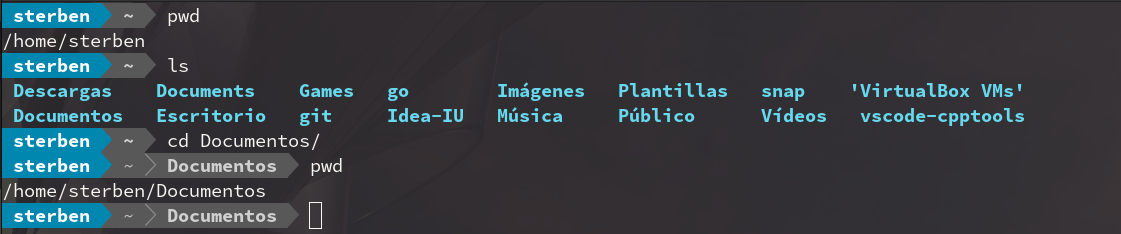
\includegraphics[width=1\textwidth]{img/navegacion.png}
\end{figure}

\newpage

\subsection{Visualización}
Existen paquetes como \textbf{tree} que permiten ver la estructura de directorios en formato de árbol.

\begin{lstlisting}
    # Install the tree package
    sudo apt install tree

    # Use the tree command to display the directory structure
    tree /path/to/directory      
\end{lstlisting}

\textbf{Nota:} El comando `apt` es un gestor de paquetes utilizado en algunas distribuciones de Linux. Dependiendo del sistema operativo que estés usando, encontrarás diferentes gestores de paquetes. El siguiente ejemplo se presenta para \textbf{Fedora 40}, que utiliza el gestor de paquetes `dnf`.

Puedes encontrar más información sobre los diferentes gestores de paquetes en Linux en este 
\href{https://www.profesionalreview.com/2016/09/11/gestor-de-paquetes-en-linux/#:~:text=DNF%20es%20el%20gestor%20de,en%20CentOS%20en%20el%20futuro.&text=Probando%20los%20diferentes%20gestores%20de,que%20te%20resulte%20m%C3%A1s%20c%C3%B3modo.}{\textcolor{blue}{enlace}}:

\subsection*{Ejemplo}
\begin{figure}[h!]
    \centering
    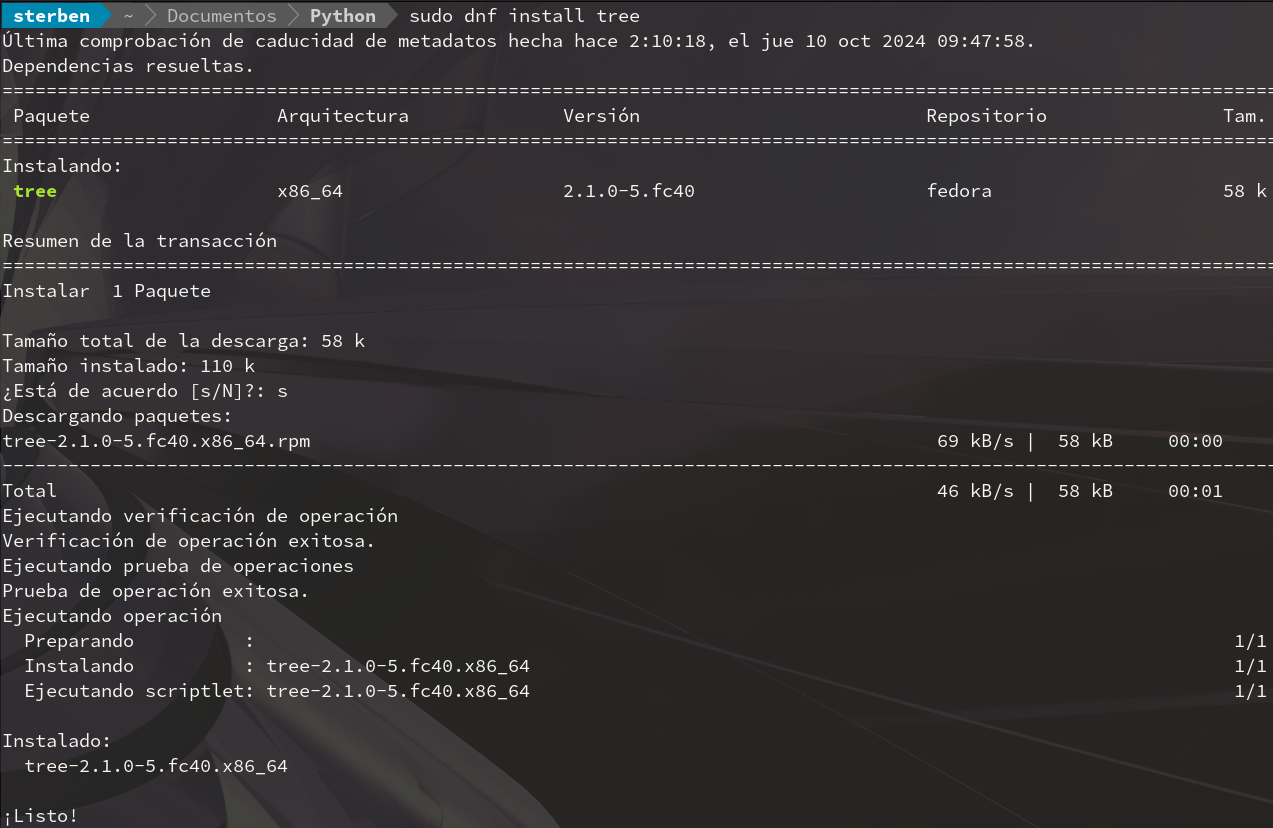
\includegraphics[width=0.8\textwidth]{img/visuali1.png}
    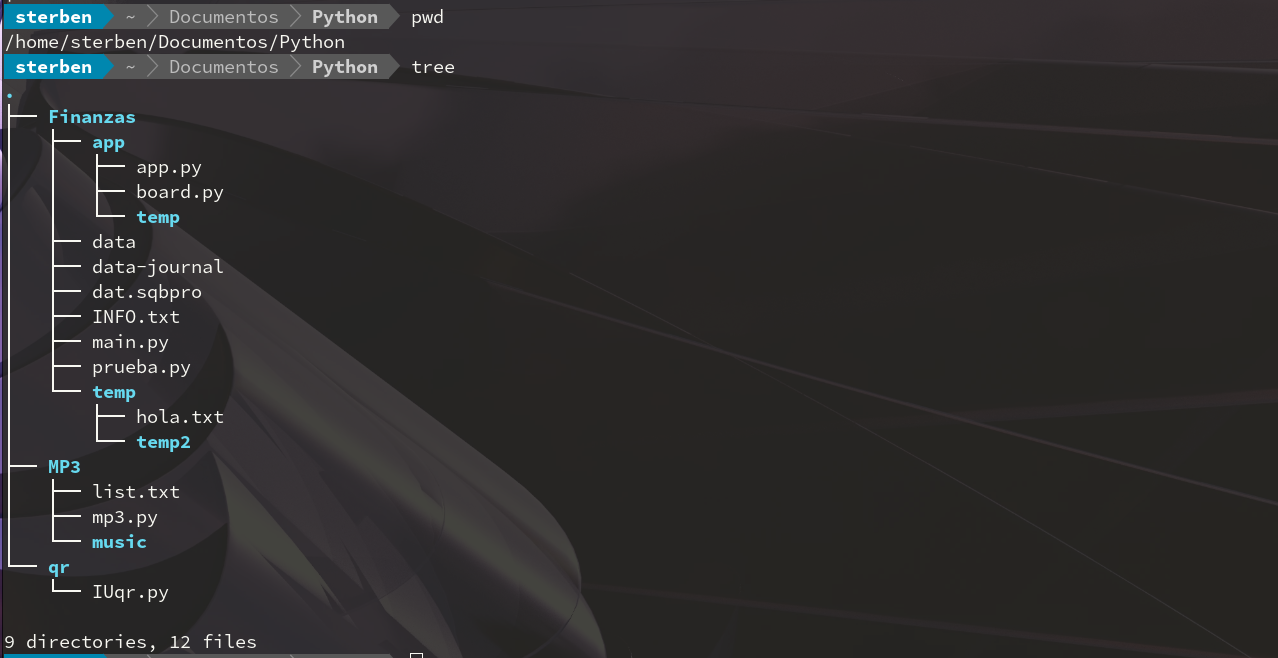
\includegraphics[width=0.8\textwidth]{img/visuali2.png}
\end{figure}

\subsection{Permisos}
En el ejemplo anterior, al instalar un paquete, se solicita la contraseña. Esto ocurre porque necesitamos permisos de \textbf{superusuario} (superUser). Además, es posible verificar los permisos de cada directorio y archivo desde la consola.

En Linux, los permisos se representan con las siguientes letras:
\begin{itemize}
    \item \textbf{d}: indica un directorio.
    \item \textbf{r}: permite la lectura.
    \item \textbf{w}: permite la escritura.
    \item \textbf{x}: permite la ejecución.
\end{itemize}

Para verificar los permisos, utilizaremos un comando que ya aprendimos, que es \textbf{ls}. Al verificar más datos con \textbf{ls --help}, podemos observar que hay opciones que nos permiten listar todos los directorios y archivos con sus respectivos permisos:

\begin{lstlisting}
    # List files and directories
    ls

    # List files and directories with detailed information 
    ls -l     

    # List all files and directories, including hidden ones, with detailed information
    ls -la
\end{lstlisting}

\subsection*{Ejemplo}
\begin{figure}[h!]
    \centering
    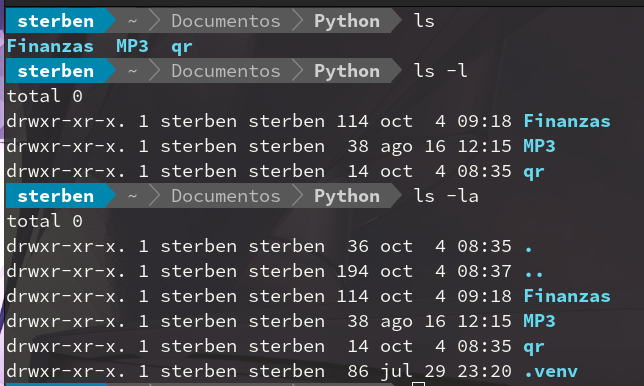
\includegraphics[width=0.9\textwidth]{img/permisos.png}
\end{figure}

\subsubsection*{Explicación}
\begin{lstlisting}
    drwxr-xr-x. 1 sterben1 sterben2 114 oct  4 09:18 Finanzas
\end{lstlisting}

\begin{itemize}
    \item \textbf{d}: directorio.
    \item \textbf{rwx}: el propietario \textbf{sterben1} tiene permisos de lectura, escritura y ejecución.
    \item \textbf{r-x}: el grupo \textbf{sterben2} tiene permisos de lectura y ejecución.
    \item \textbf{r-x}: otros (también \textbf{sterben2}) tienen permisos de lectura y ejecución.
    \item \textbf{114}: tamaño en bytes (no representa el valor real).
    \item \textbf{oct 4 09:18}: fecha de la última modificación.
    \item \textbf{Finanzas}: nombre del directorio.
\end{itemize}

\section{Gestor de Archivos y Directorios}
En este apartado, veremos operaciones básicas como copiar, mover, eliminar o crear diferentes archivos y directorios.

\begin{lstlisting}
    # Copy a file to a specific destination
    cp archivo destino

    # Move a file to a new destination, renaming it if necessary
    mv archivo destino     

    # Remove a file
    rm archivo

    # Create a new directory
    mkdir nombreDirectorio

    # Remove an empty directory
    rmdir nombreDirectorio
\end{lstlisting}

\chapter{Windows}

\section{Navegacion entre Directorios}
    Los codigos principales en esta sección seria: 
    \begin{lstlisting}
        # Revisar el directorio actual
        cd
        # Listar archivos y directorios
        dir
        # Cambiar al directorio especificado
        cd C:\ruta\al\directorio        
    \end{lstlisting}



    
\end{document}
